%%%%%%%%%%%%%%%%%%%%%%%%%%%%%%%%%%%%%%%%%
% Memo
% LaTeX Template
% Version 1.0 (30/12/13)
%
% This template has been downloaded from:
% http://www.LaTeXTemplates.com O Original author:
% Rob Oakes (http://www.oak-tree.us) with modifications by:
% Vel (vel@latextemplates.com)
%
% License:
% CC BY-NC-SA 3.0 (http://creativecommons.org/licenses/by-nc-sa/3.0/)
%
%%%%%%%%%%%%%%%%%%%%%%%%%%%%%%%%%%%%%%%%%

\documentclass[a4paper,12pt]{texMemo} % Set the paper size (letterpaper, a4paper, etc) and font size (10pt, 11pt or 12pt)
\usepackage{setspace}
\usepackage{parskip} % Adds spacing between paragraphs
\usepackage{graphicx}
\usepackage{geometry}
\setlength{\parindent}{15pt} % Indent paragraphs

%----------------------------------------------------------------------------------------
%	MEMO INFORMATION
%----------------------------------------------------------------------------------------

\memoto{Decision Maker about Privacy} % Recipient(s)

\memofrom{MCM 2018 Team} % Sender(s)

\memosubject{Private Information: The Emergence of a New Asset} % Memo subject

\memodate{Monday, February 12, 2018} % Date, set to \today for automatically printing todays date

%\logo{\includegraphics[width=0.3\textwidth]{logo.png}} % Institution logo at the top right of the memo, comment out this line for no logo

%----------------------------------------------------------------------------------------

\begin{document}

\maketitle % Print the memo header information

%----------------------------------------------------------------------------------------
%	MEMO CONTENT
%----------------------------------------------------------------------------------------

\section{Introduction}
In the era of "anywhere, anytime",  people now produce more data than ever before. The variety and volume of digital records that can be created, processed and analyzed will continue to increase dramatically. By 2020, International Data Corporation (IDC) estimates that the global amount of digital records will increase more than 40-fold. 

The problem is to quantify the cost of privacy. That is, to establish a metric to evaluate the monetary value of keeping PI protected and the fees it would cost for others to possess or utilize PI. We consider private information (PI) as record of "everything a person makes and does". To make the problem clearer, several concepts need to be explained.
%\begin{spacing}{0.8}

\textbf{Domain of Private Information.}   An initial list of types of private information includes:
Digital identity (e.g., names, addresses, phone numbers, demographic information, social network profile information, etc.); Relationships to other people and organization (social media, contact list and profiles); Communication data and logs (emails, SMS, phone calls, IM and social network posts); Media produced, consumed and shared (in-text, audio, photo, video and other forms of media); Financial data (financial transactions, accounts, credit scores, physical assets and virtual goods); Health data (health/medical records, medical history, medical device logs, prescriptions and health insurance coverage); Institutional data (government, academic and employment data).
%\end{spacing} 

\textbf{Subgroup of Individuals.} E.g. citizenship, professional profiles, age, education level, occupation, etc.

\textbf{Risks.} The risks involve loss of safety, money, valuable items, intellectual property (IP),  the person's electronic identity, professional embarrassment , loss of a position or job, social loss (friendships), social stigmatization, or marginalization.
\section{Solutions and Conclusions}
\begin{figure}
\begin{center}
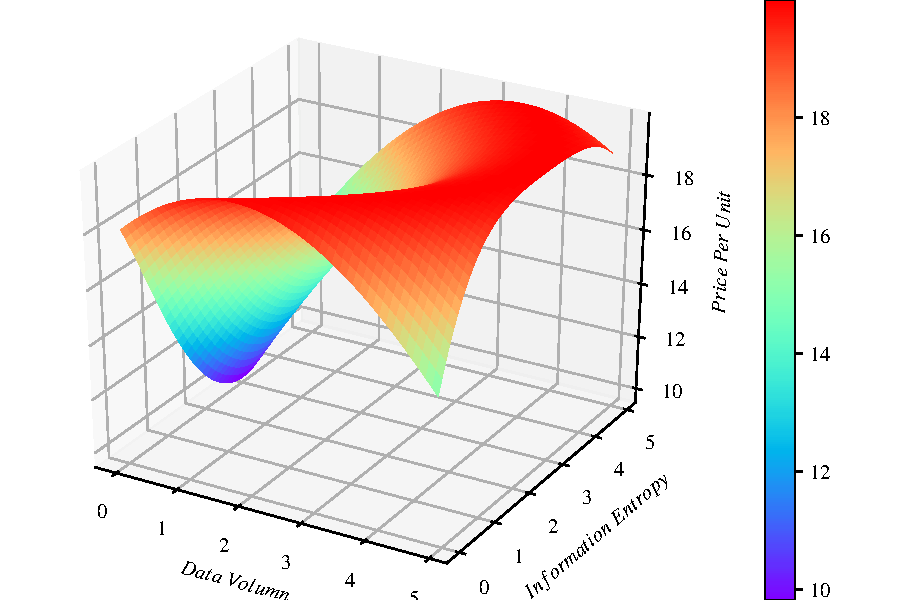
\includegraphics[width=0.7\linewidth]{fig/demand_surface.pdf}
\caption{Demand Surface: the influence of data volumn and information entropy}
\end{center}
\end{figure}


Private information will continue to increase dramatically in both quality and diversity, and has the potential to unlock significant economic and societal value.
To some extend, Private Information (PI) is similar to personal property (PP) and intellectual property (IP). However, there are also discrepancies among them. PI differs from PP and IP in that it can be sold or given to others who then have the right to use it without ownership, and it needs to be regulated by government. These information and privacy issues should be protected not only by the individuals but also by the agencies. Based on our model, the private data should not be trackable by the government for national security concerns.

%Potential gains from keeping data private include a greater level of security, especially for larger businesses. Potential losses from keeping data private include slowing down the pace of technological development. Notably, currently the development of \emph{Artificial Intelligence} can not make such a big achievement without big data, e.g. ImageNet. Also, public sectors can trace the spread of disease in order to prevent further outbreak with shared private information, which is a welfare for most people. Commercial agencies can provide personalized service for different groups.

Building a harmonious ecosystem around personal data will require significant commitment from all stakeholders. Our model proposes four critical solutions to deal with the problem:
\begin{itemize}
\item An expanded role for government, such that governments can use their purchasing power to help shape commercially available products and solutions that the private sector can then leverage;
\item Mechanisms for enhancing trust among all parts in private information transaction;
%\item Greater interoperability among existing data silos;
%\item An easy-to-understand user-centric approach to the design of systems, tools and policies, with an emphasis on transparency, trust, control and value distribution.

\item Integrate principles surrounding and user trust and data protection into the development of new services and platforms;
%\item Engage with leading innovators and end user advocacy groups to explore the further applications for, and development of, trust framework;
\item Policy makers and agencies should launch an international dialog, which should encompass governments, international bodies such as the World Trade Organization, end user privacy rights groups and representation from the private sector. It should include not only US and European Union members, but interested parties from the Asia-Pacific region and emerging countries;
%\item In the United States: Agencies should closely watch developments of the National Strategy for Trusted Identities in Cyberspace program and the privacy bill. Agencies need to be in constant dialog with the US Department of Commerce, the Federal Trade Commission and other bodies to help shape future legislation and policies; In the European Union: Agencies should collaborate with the European Commission in its move to revise the EU privacy directive. In other regions that differ from the US or the EU in cultural or social norms, very different paths in adopting policy frameworks will be required. One initial step in making progress could be to seek ways to harmonize fragmented national privacy policies.
\end{itemize}

%----------------------------------------------------------------------------------------

\end{document}